\section{Stream mining software}
\label{State::StreamMining}

Data stream mining is a relatively new field. Even though its theoretical foundation is based in well-established statistical and computational approaches, it has not been until recent years that this research area has experimented a great growth in interest~\citet{Gaber:MiningDataStreamsReview}.

Because it is an incipient field, stream mining software packages are quite uncommon. Even though specific applications have been developed (see~\citet{Kargupta:MineFleet}), MOA remains as one of the few generic, free and open sourced systems. One example of a commercial solution that includes support for data stream mining is RapidMiner, through the use of plugins. 

MOA is currently the most complete framework for data stream clustering research and it is an important pioneer in experimenting with data stream algorithms. MOA's advantages are that it interfaces with WEKA, provides already a set of data stream classification and clustering algorithms and it has a clear Java interface to add new algorithms or use the existing algorithms in other applications.

Related to MOA, a new project called SAMOA (from Scalable Advanced Massive Online Analysis) is being developed too, based on MOA itself and a couple of streaming processing engines: Apache S4~\citep{web:ApacheS4} and Apache Storm~\citep{web:ApacheStorm}, developed by the Apache Software Foundation.

Finally, an R package called \texttt{stream} was released into the CRAN repository\footnote{The capabilities of the R language are extended through user-created packages. Most of these packages are available at the Comprehensive R Archive Network (CRAN), on the following web address: \url{http://cran.r-project.org}.} in 2013. It allows to do real time analytics on data streams and is currently focused on clustering algorithms available in MOA.

\subsection{The MOA framework}

Massive Online Analysis (MOA) is a software environment for implementing algorithms and running experiments for online learning from evolving data streams. MOA is designed to deal with the challenging problems of scaling up the implementation of state of the art algorithms to real world dataset sizes and of making algorithms comparable in benchmark streaming settings.

MOA contains a collection of offline and online algorithms for both classification and clustering as well as tools for evaluation. Researchers benefit from MOA by getting insights into workings and problems of different approaches, practitioners can easily compare several algorithms and apply them to real world data sets and settings.

\begin{figure}
\centering
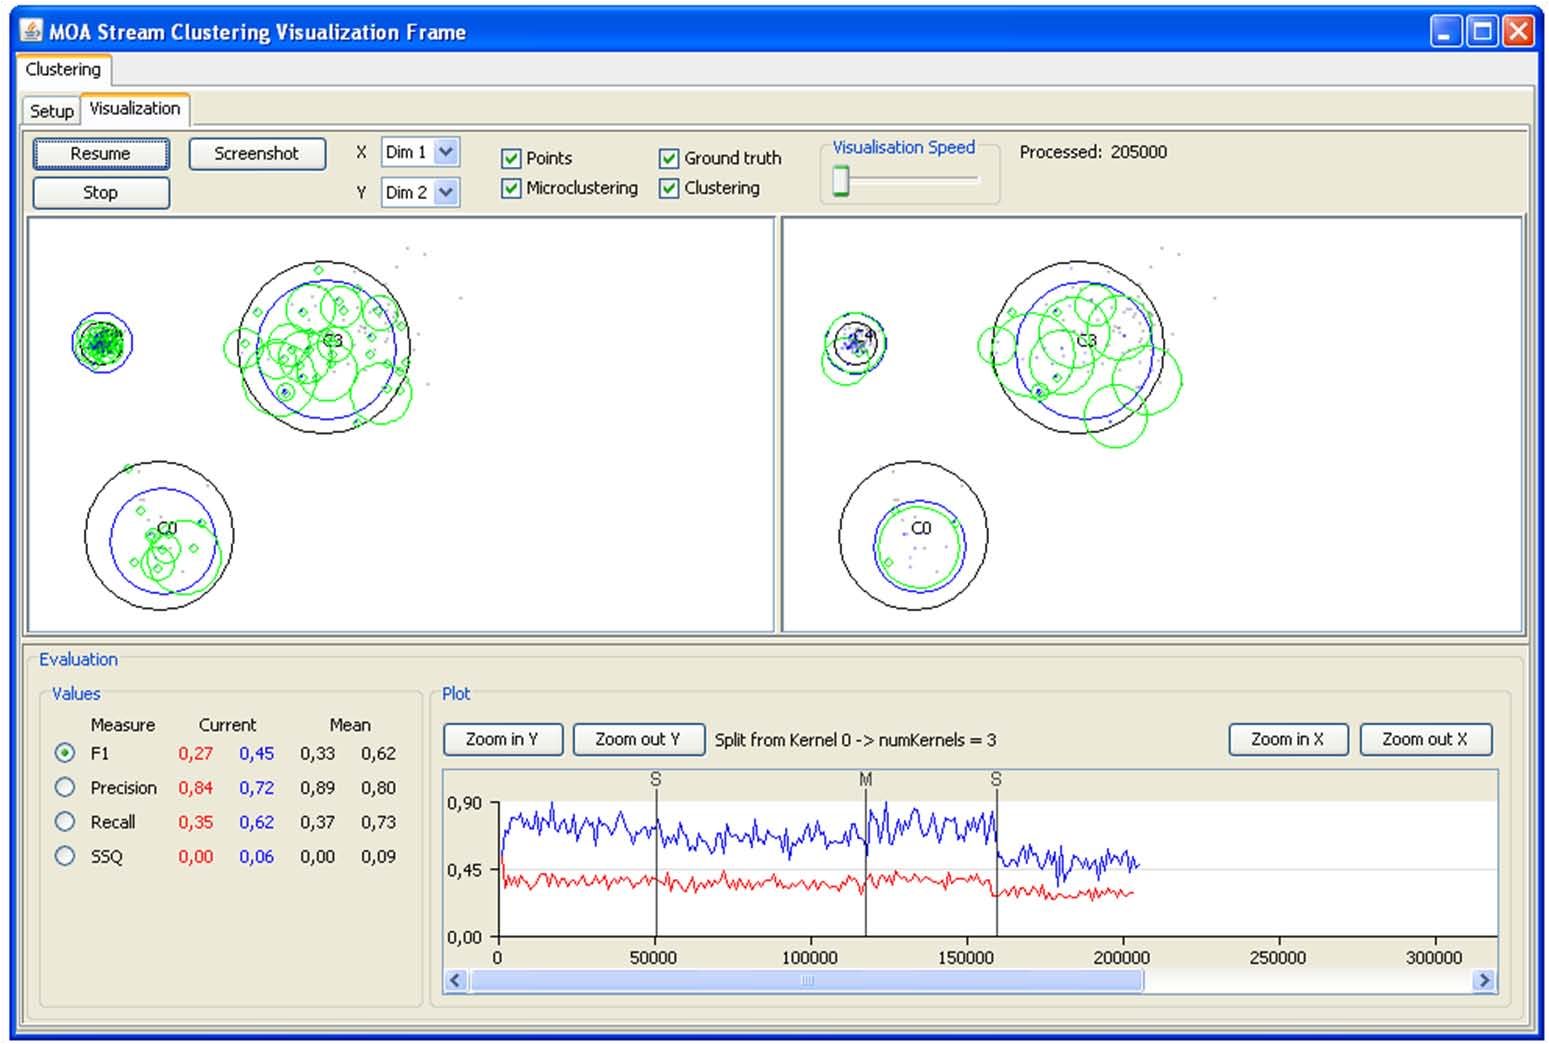
\includegraphics[width=0.7\linewidth]{figures/moa-gui-2.png}
\caption[MOA's Graphical User Interface]{MOA's Graphical User Interface, showing the clustering visualization capabilities of the software.}
\end{figure}

MOA supports bi-directional interaction with WEKA, the Waikato Environment for Knowledge Analysis, which is an award-winning open-source workbench containing implementations of a wide range of batch machine learning methods. WEKA is also written in Java. The main benefits of Java are portability, where applications can be run on any platform with an appropriate Java virtual machine, and the strong and well-developed support libraries. Use of the language is widespread, and features such as the automatic garbage collection help to reduce programmer burden and error.

The MOA framework provides a graphical user interface (GUI), which eases its use, when experiments can be carried out using the algorithms already included in the framework. However, for more complicated analysis or industry-scaled uses, MOA offers the possibility to be used using a command line interface, which is extremely powerful and flexible. Also, due to its open source nature and the fact that it is built in Java, custom procedures and integration techniques can be developed to meet the data analysis requirements. Last but not least, when the core features are not sufficient for the user's needs, MOA can be extended with new mining algorithms, new stream generators or evaluation measures, like the SDC filters that we will implement in this project.